\chapter{Signal processing}
In this chapter, we look at the basics of signal processing and how it
relates to signal modulation, demodulation and decoding of information
in \gls{GSM} communication. Such signals on the Um air interface in
GSM are quadrature modulated using \gls{GMSK}.\ In this type of
modulation, bits are mapped to symbols, pulse shaped by a gaussian
filter and carried pairwise by two orthogonal signals, $90^{\circ}$
degrees apart. These signals are combined into a final signal,
$v \para{t}$, ready to be transmitted. Modulation schemes can carry
symbol information by shifts in frequency, phase and amplitude. The
\gls{GMSK} modulation scheme changes its phase in a continuous matter which
reduces the required bandwidth compared to an abrupt change as in the
phase shift keying modulation scheme.

It follows from Euler's equation that a complex number in polar form
is dependent on the phase angle, $\phi$, and can be represented as the
sum of cosine- and sine functions of phase angle, where cosine is the
real part and sine is the imaginary part,

\begin{equation}
  e^{i \phi} = \cos \para{\phi} + i \sin \para{\phi}, \quad \phi \in \mathbb{R}.
\end{equation}

\cref{fig:phasor_diagram} illustrates a so-called harmonic phasor of a
signal, a complex number in polar form, and its real and imaginary
parts which are made of two real orthogonal signals as a cosine- and a
sine function. The amplitude of these two individual signals are
referred to as a complex signal's \gls{I}-, and \gls{Q}-, components
and they are important quantities in quadrature modulation. In fact,
the modulated final signal, $v \para{t}$, can be identified as a
complex signal made of its two orthogonal signal components. Hence the
name quadrature modulation.

\begin{figure}
  \centering
  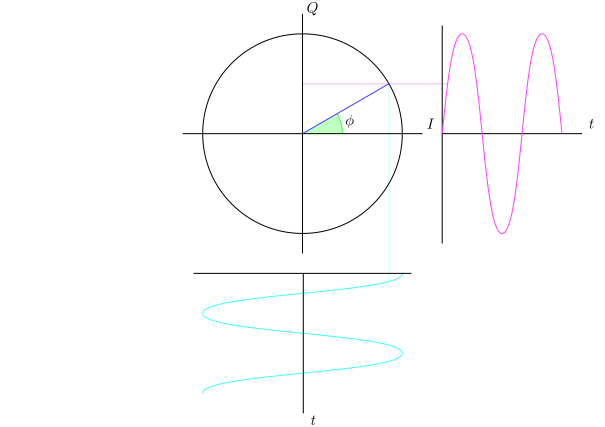
\includegraphics[width=0.7\textwidth]{figures/phasor_diagram}
  \caption{I/Q phasor plot of a complex signal made of two
    real signals, $90^{\circ}$ degrees apart.}
  \label{fig:phasor_diagram}
\end{figure}

In modulation schemes, a number of bits are mapped to one symbol e.g.\
\gls{BPSK}, and G/MSK map just a single bit and an element in such a
binary data sequence of length $k$ at index $i$ can be described as

\begin{equation}
  d_i \in \left\{ 0, 1\right\}^k.
\end{equation}

In the same sense, symbols $D_i$ can be mapped directly to elements in
the binary data sequence as

\begin{equation}
  D_i = \begin{cases}
    +1 & \mbox{if } d_i = 1,\\
    -1 & \mbox{if } d_i = 0,
  \end{cases} \quad i = 1, \dots, k.
\end{equation}

Symbols are used to better recognize zero values, at which a regular
digital square wave has no zero crossings. It is difficult in the
analysis of an analog signal to distinguish between a sequence of
digital zeros and no transmission at all~\cite[p. 157]{onion}.

The symbol mapping is one step towards the modulation of a signal.

\section{Modulation}
Modulation comes in many shapes and its purpose is typically to carry
information in an analog signal by varying the signal's phase,
frequency or amplitude. To fulfill these requirements a radio system
must convert the information to a format that can be carried by radio
waves. In \gls{GSM}, the information is given by a binary sequence, mapped
to symbols, which must be modulated such that the receiver is able to
translate and receive the original message.

A square wave that crosses zero is still not optimal, since such a
signal requires high frequencies to shape its steep transitions. Its
Fourier transform results in a $\sinc$ function in the frequency
domain that is unlimited in bandwidth. The binary data must therefore
be shaped into a different signal to limit the bandwidth. This process
is called \textit{pulse shaping} where a digital signal is convolved
into an analog signal through a pulse shaping filter. The $\sinc$ can
be applied to such convolution of a digital signal which results in a
very narrow and sharp bandwidth of low frequencies. In communication
systems, this phenomena is ideal since it increases the amount of
carriers which equals more channels in an \gls{FDMA} aspect.

Another important situation that must be considered when choosing the
pulse shape filter, is how a sequence of symbols will be transmitted
continuously. The $\sinc$ function convolved with the symbols over a
time interval cause adjacent symbols to overlap. This situation is
called \gls{ISI}, and it makes symbols difficult to restore. For this
reason, the type of filter is chosen based on the specific
application.

With two streams of pulse-shaped symbols in quadrature modulation, the
modulated signal, $v \para{t}$, can be expressed as
\begin{equation}
  v \para{t} =
  m_1 \para{t} \sqrt{2}\cos \para{2 \pi f_c t} -
  m_2 \para{t} \sqrt{2}\sin \para{2 \pi f_c t}
\label{eq:modulated_signal}
\end{equation}
where
\begin{itemize}[labelindent=\parindent]
\item[$m_1, m_2$] are the message streams of pulse-shaped symbols and
\item[$f_c$] is the carrier frequency~\cite[p. 102]{onion}.
\end{itemize}

\cref{eq:modulated_signal} is illustrated in
\cref{fig:signal_generation_diagram}.

\begin{figure}
  \centering
  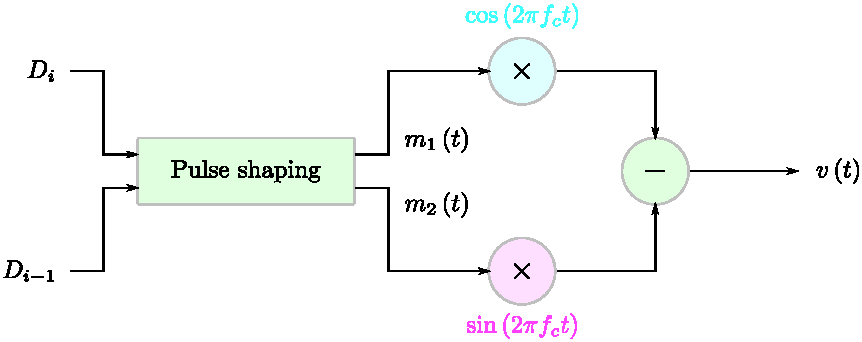
\includegraphics[width=0.7\textwidth]{figures/signal_generation_diagram}
  \caption{Digital to analog signal conversion with quadrature modulation.}
  \label{fig:signal_generation_diagram}
\end{figure}
\subsection{Gaussian minimum shift keying}
% NOTE: Maybe include phase diagram over symbol time to show smooth
% transitions over 3T
%
% Constellation diagram perhaps?
\gls{GSM} uses the \gls{GMSK} modulation scheme that is a combination
of \gls{MSK} modulation and a gaussian filter used for shaping the
symbol pulse. Both \gls{GMSK} and \gls{MSK} avoid abrupt changes in
the signal by smoothly changing the phase over time for each
transmitted symbol. This behavior is known as a continuous phase
scheme and it gives no discontinuity in the signal and reduces the
required bandwidth. Since the information is carried in phase, the
symbols are redefined and further mapped to constellation points, as
illustrated in \cref{fig:constellation_diagram}, in a complex plane

\begin{equation}
  S_i = j \cdot D_i \cdot D_{i - 1} \cdot S_{i - 1}.
  \label{eq:msk_mapping}
\end{equation}

$S_0$ is initially set to $1$ unless specified otherwise and the new
mappings are later used for estimation of a symbol sequence.

\begin{figure}
  \centering
  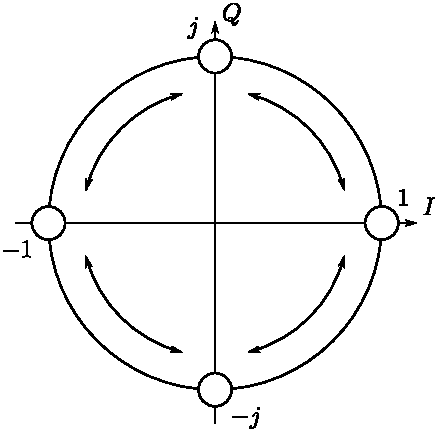
\includegraphics[width=0.4\textwidth]{figures/constellation_diagram}
  \caption{Symbols mapped to $\pi/2$ rotations over time as expressed by
    \cref{eq:msk_mapping}.}
  \label{fig:constellation_diagram}
\end{figure}

The gaussian filter shapes the symbols to stretch slightly longer in
time, but it further reduces the signal's bandwidth. In fact, its time
response is infinite and it is therefore truncated.

The \gls{GSM} standard specifies a pulse shape of the gaussian function,
$h \para{t}$, in \cref{eq:gaussian} with $BT = 0.3$. $T$ is the symbol
period at $3.69\si{\mu s}$ and $B$ refers to the bandwidth of gaussian
filter. By increasing the bandwidth, $B$, with $T$ declared constant,
the shape begins to relate to MSK~\cite[p. 5--7]{modulation}.\
\begin{equation}
  \begin{aligned}
    \delta &= \dfrac{\sqrt{\ln \para{2}}}{2 \pi BT}\\
    h \para{t} &=
    \dfrac{1}{\sqrt{2 \pi} \delta T}
    e^{-t^2 / \para{2 \delta^2 T^2}}.
  \end{aligned}
  \label{eq:gaussian}
\end{equation}

As \cref{fig:gaussian} illustrates, the gaussian function's growth
varies with the value of the $BT$ product. By adding a sequence of
this growth with a symbol duration width of $T$, it is easily thought
to cause trouble if the shape is too wide and that its frequency
response widens as the shape gets thinner.

With a fully modulated signal, the process must also be invertable at
the receiver which is part of the sampling process.

\begin{figure}[H]
  \centering
  \begin{tikzpicture}[gnuplot]
%% generated with GNUPLOT 5.0p0 (Lua 5.2; terminal rev. 99, script rev. 100)
%% Thu Jun 11 15:47:53 2015
\path (0.000,0.000) rectangle (12.500,5.000);
\gpcolor{color=gp lt color border}
\gpsetlinetype{gp lt border}
\gpsetdashtype{gp dt solid}
\gpsetlinewidth{1.00}
\draw[gp path] (1.012,0.985)--(1.192,0.985);
\draw[gp path] (11.947,0.985)--(11.767,0.985);
\node[gp node right] at (0.828,0.985) {$0$};
\draw[gp path] (1.012,1.714)--(1.192,1.714);
\draw[gp path] (11.947,1.714)--(11.767,1.714);
\node[gp node right] at (0.828,1.714) {$0.2$};
\draw[gp path] (1.012,2.443)--(1.192,2.443);
\draw[gp path] (11.947,2.443)--(11.767,2.443);
\node[gp node right] at (0.828,2.443) {$0.4$};
\draw[gp path] (1.012,3.173)--(1.192,3.173);
\draw[gp path] (11.947,3.173)--(11.767,3.173);
\node[gp node right] at (0.828,3.173) {$0.6$};
\draw[gp path] (1.012,3.902)--(1.192,3.902);
\draw[gp path] (11.947,3.902)--(11.767,3.902);
\node[gp node right] at (0.828,3.902) {$0.8$};
\draw[gp path] (1.012,4.631)--(1.192,4.631);
\draw[gp path] (11.947,4.631)--(11.767,4.631);
\node[gp node right] at (0.828,4.631) {$1$};
\draw[gp path] (1.012,0.985)--(1.012,1.165);
\draw[gp path] (1.012,4.631)--(1.012,4.451);
\node[gp node center] at (1.012,0.677) {$-10$};
\draw[gp path] (3.746,0.985)--(3.746,1.165);
\draw[gp path] (3.746,4.631)--(3.746,4.451);
\node[gp node center] at (3.746,0.677) {$-5$};
\draw[gp path] (6.480,0.985)--(6.480,1.165);
\draw[gp path] (6.480,4.631)--(6.480,4.451);
\node[gp node center] at (6.480,0.677) {$0$};
\draw[gp path] (9.213,0.985)--(9.213,1.165);
\draw[gp path] (9.213,4.631)--(9.213,4.451);
\node[gp node center] at (9.213,0.677) {$5$};
\draw[gp path] (11.947,0.985)--(11.947,1.165);
\draw[gp path] (11.947,4.631)--(11.947,4.451);
\node[gp node center] at (11.947,0.677) {$10$};
\draw[gp path] (1.012,4.631)--(1.012,0.985)--(11.947,0.985)--(11.947,4.631)--cycle;
\node[gp node center] at (6.479,0.215) {Time $\sq{\mu s}$};
\node[gp node right] at (10.479,4.297) {$BT = 0.1$};
\gpcolor{rgb color={0.580,0.000,0.827}}
\draw[gp path] (10.663,4.297)--(11.579,4.297);
\draw[gp path] (1.012,1.022)--(1.039,1.023)--(1.067,1.023)--(1.094,1.024)--(1.122,1.025)%
  --(1.149,1.026)--(1.176,1.027)--(1.204,1.027)--(1.231,1.028)--(1.259,1.029)--(1.286,1.030)%
  --(1.313,1.031)--(1.341,1.032)--(1.368,1.033)--(1.396,1.034)--(1.423,1.035)--(1.450,1.036)%
  --(1.478,1.037)--(1.505,1.038)--(1.533,1.039)--(1.560,1.040)--(1.588,1.041)--(1.615,1.042)%
  --(1.642,1.043)--(1.670,1.044)--(1.697,1.045)--(1.725,1.046)--(1.752,1.047)--(1.779,1.048)%
  --(1.807,1.050)--(1.834,1.051)--(1.862,1.052)--(1.889,1.053)--(1.916,1.054)--(1.944,1.056)%
  --(1.971,1.057)--(1.999,1.058)--(2.026,1.059)--(2.053,1.061)--(2.081,1.062)--(2.108,1.063)%
  --(2.136,1.064)--(2.163,1.066)--(2.190,1.067)--(2.218,1.068)--(2.245,1.070)--(2.273,1.071)%
  --(2.300,1.073)--(2.327,1.074)--(2.355,1.075)--(2.382,1.077)--(2.410,1.078)--(2.437,1.080)%
  --(2.465,1.081)--(2.492,1.083)--(2.519,1.084)--(2.547,1.086)--(2.574,1.087)--(2.602,1.089)%
  --(2.629,1.090)--(2.656,1.092)--(2.684,1.094)--(2.711,1.095)--(2.739,1.097)--(2.766,1.098)%
  --(2.793,1.100)--(2.821,1.102)--(2.848,1.103)--(2.876,1.105)--(2.903,1.107)--(2.930,1.108)%
  --(2.958,1.110)--(2.985,1.112)--(3.013,1.113)--(3.040,1.115)--(3.067,1.117)--(3.095,1.118)%
  --(3.122,1.120)--(3.150,1.122)--(3.177,1.124)--(3.204,1.125)--(3.232,1.127)--(3.259,1.129)%
  --(3.287,1.131)--(3.314,1.133)--(3.342,1.134)--(3.369,1.136)--(3.396,1.138)--(3.424,1.140)%
  --(3.451,1.142)--(3.479,1.143)--(3.506,1.145)--(3.533,1.147)--(3.561,1.149)--(3.588,1.151)%
  --(3.616,1.153)--(3.643,1.154)--(3.670,1.156)--(3.698,1.158)--(3.725,1.160)--(3.753,1.162)%
  --(3.780,1.164)--(3.807,1.166)--(3.835,1.167)--(3.862,1.169)--(3.890,1.171)--(3.917,1.173)%
  --(3.944,1.175)--(3.972,1.177)--(3.999,1.178)--(4.027,1.180)--(4.054,1.182)--(4.081,1.184)%
  --(4.109,1.186)--(4.136,1.188)--(4.164,1.189)--(4.191,1.191)--(4.219,1.193)--(4.246,1.195)%
  --(4.273,1.197)--(4.301,1.198)--(4.328,1.200)--(4.356,1.202)--(4.383,1.204)--(4.410,1.205)%
  --(4.438,1.207)--(4.465,1.209)--(4.493,1.211)--(4.520,1.212)--(4.547,1.214)--(4.575,1.216)%
  --(4.602,1.217)--(4.630,1.219)--(4.657,1.221)--(4.684,1.222)--(4.712,1.224)--(4.739,1.226)%
  --(4.767,1.227)--(4.794,1.229)--(4.821,1.230)--(4.849,1.232)--(4.876,1.234)--(4.904,1.235)%
  --(4.931,1.237)--(4.958,1.238)--(4.986,1.239)--(5.013,1.241)--(5.041,1.242)--(5.068,1.244)%
  --(5.095,1.245)--(5.123,1.247)--(5.150,1.248)--(5.178,1.249)--(5.205,1.251)--(5.233,1.252)%
  --(5.260,1.253)--(5.287,1.254)--(5.315,1.256)--(5.342,1.257)--(5.370,1.258)--(5.397,1.259)%
  --(5.424,1.260)--(5.452,1.261)--(5.479,1.262)--(5.507,1.263)--(5.534,1.264)--(5.561,1.265)%
  --(5.589,1.266)--(5.616,1.267)--(5.644,1.268)--(5.671,1.269)--(5.698,1.270)--(5.726,1.271)%
  --(5.753,1.272)--(5.781,1.272)--(5.808,1.273)--(5.835,1.274)--(5.863,1.275)--(5.890,1.275)%
  --(5.918,1.276)--(5.945,1.277)--(5.972,1.277)--(6.000,1.278)--(6.027,1.278)--(6.055,1.279)%
  --(6.082,1.279)--(6.110,1.280)--(6.137,1.280)--(6.164,1.280)--(6.192,1.281)--(6.219,1.281)%
  --(6.247,1.281)--(6.274,1.282)--(6.301,1.282)--(6.329,1.282)--(6.356,1.282)--(6.384,1.282)%
  --(6.411,1.282)--(6.438,1.282)--(6.466,1.282)--(6.493,1.282)--(6.521,1.282)--(6.548,1.282)%
  --(6.575,1.282)--(6.603,1.282)--(6.630,1.282)--(6.658,1.282)--(6.685,1.282)--(6.712,1.281)%
  --(6.740,1.281)--(6.767,1.281)--(6.795,1.280)--(6.822,1.280)--(6.849,1.280)--(6.877,1.279)%
  --(6.904,1.279)--(6.932,1.278)--(6.959,1.278)--(6.987,1.277)--(7.014,1.277)--(7.041,1.276)%
  --(7.069,1.275)--(7.096,1.275)--(7.124,1.274)--(7.151,1.273)--(7.178,1.272)--(7.206,1.272)%
  --(7.233,1.271)--(7.261,1.270)--(7.288,1.269)--(7.315,1.268)--(7.343,1.267)--(7.370,1.266)%
  --(7.398,1.265)--(7.425,1.264)--(7.452,1.263)--(7.480,1.262)--(7.507,1.261)--(7.535,1.260)%
  --(7.562,1.259)--(7.589,1.258)--(7.617,1.257)--(7.644,1.256)--(7.672,1.254)--(7.699,1.253)%
  --(7.726,1.252)--(7.754,1.251)--(7.781,1.249)--(7.809,1.248)--(7.836,1.247)--(7.864,1.245)%
  --(7.891,1.244)--(7.918,1.242)--(7.946,1.241)--(7.973,1.239)--(8.001,1.238)--(8.028,1.237)%
  --(8.055,1.235)--(8.083,1.234)--(8.110,1.232)--(8.138,1.230)--(8.165,1.229)--(8.192,1.227)%
  --(8.220,1.226)--(8.247,1.224)--(8.275,1.222)--(8.302,1.221)--(8.329,1.219)--(8.357,1.217)%
  --(8.384,1.216)--(8.412,1.214)--(8.439,1.212)--(8.466,1.211)--(8.494,1.209)--(8.521,1.207)%
  --(8.549,1.205)--(8.576,1.204)--(8.603,1.202)--(8.631,1.200)--(8.658,1.198)--(8.686,1.197)%
  --(8.713,1.195)--(8.740,1.193)--(8.768,1.191)--(8.795,1.189)--(8.823,1.188)--(8.850,1.186)%
  --(8.878,1.184)--(8.905,1.182)--(8.932,1.180)--(8.960,1.178)--(8.987,1.177)--(9.015,1.175)%
  --(9.042,1.173)--(9.069,1.171)--(9.097,1.169)--(9.124,1.167)--(9.152,1.166)--(9.179,1.164)%
  --(9.206,1.162)--(9.234,1.160)--(9.261,1.158)--(9.289,1.156)--(9.316,1.154)--(9.343,1.153)%
  --(9.371,1.151)--(9.398,1.149)--(9.426,1.147)--(9.453,1.145)--(9.480,1.143)--(9.508,1.142)%
  --(9.535,1.140)--(9.563,1.138)--(9.590,1.136)--(9.617,1.134)--(9.645,1.133)--(9.672,1.131)%
  --(9.700,1.129)--(9.727,1.127)--(9.755,1.125)--(9.782,1.124)--(9.809,1.122)--(9.837,1.120)%
  --(9.864,1.118)--(9.892,1.117)--(9.919,1.115)--(9.946,1.113)--(9.974,1.112)--(10.001,1.110)%
  --(10.029,1.108)--(10.056,1.107)--(10.083,1.105)--(10.111,1.103)--(10.138,1.102)--(10.166,1.100)%
  --(10.193,1.098)--(10.220,1.097)--(10.248,1.095)--(10.275,1.094)--(10.303,1.092)--(10.330,1.090)%
  --(10.357,1.089)--(10.385,1.087)--(10.412,1.086)--(10.440,1.084)--(10.467,1.083)--(10.494,1.081)%
  --(10.522,1.080)--(10.549,1.078)--(10.577,1.077)--(10.604,1.075)--(10.632,1.074)--(10.659,1.073)%
  --(10.686,1.071)--(10.714,1.070)--(10.741,1.068)--(10.769,1.067)--(10.796,1.066)--(10.823,1.064)%
  --(10.851,1.063)--(10.878,1.062)--(10.906,1.061)--(10.933,1.059)--(10.960,1.058)--(10.988,1.057)%
  --(11.015,1.056)--(11.043,1.054)--(11.070,1.053)--(11.097,1.052)--(11.125,1.051)--(11.152,1.050)%
  --(11.180,1.048)--(11.207,1.047)--(11.234,1.046)--(11.262,1.045)--(11.289,1.044)--(11.317,1.043)%
  --(11.344,1.042)--(11.371,1.041)--(11.399,1.040)--(11.426,1.039)--(11.454,1.038)--(11.481,1.037)%
  --(11.509,1.036)--(11.536,1.035)--(11.563,1.034)--(11.591,1.033)--(11.618,1.032)--(11.646,1.031)%
  --(11.673,1.030)--(11.700,1.029)--(11.728,1.028)--(11.755,1.027)--(11.783,1.027)--(11.810,1.026)%
  --(11.837,1.025)--(11.865,1.024)--(11.892,1.023)--(11.920,1.023)--(11.947,1.022);
\gpcolor{color=gp lt color border}
\node[gp node right] at (10.479,3.989) {$BT = 0.3$};
\gpcolor{rgb color={0.000,0.620,0.451}}
\gpsetlinewidth{3.00}
\draw[gp path] (10.663,3.989)--(11.579,3.989);
\draw[gp path] (1.012,0.985)--(1.039,0.985)--(1.067,0.985)--(1.094,0.985)--(1.122,0.985)%
  --(1.149,0.985)--(1.176,0.985)--(1.204,0.985)--(1.231,0.985)--(1.259,0.985)--(1.286,0.985)%
  --(1.313,0.985)--(1.341,0.985)--(1.368,0.985)--(1.396,0.985)--(1.423,0.985)--(1.450,0.985)%
  --(1.478,0.985)--(1.505,0.985)--(1.533,0.985)--(1.560,0.985)--(1.588,0.985)--(1.615,0.985)%
  --(1.642,0.985)--(1.670,0.985)--(1.697,0.985)--(1.725,0.985)--(1.752,0.985)--(1.779,0.985)%
  --(1.807,0.985)--(1.834,0.985)--(1.862,0.985)--(1.889,0.985)--(1.916,0.985)--(1.944,0.985)%
  --(1.971,0.985)--(1.999,0.985)--(2.026,0.985)--(2.053,0.985)--(2.081,0.985)--(2.108,0.985)%
  --(2.136,0.985)--(2.163,0.985)--(2.190,0.985)--(2.218,0.985)--(2.245,0.985)--(2.273,0.985)%
  --(2.300,0.985)--(2.327,0.985)--(2.355,0.985)--(2.382,0.985)--(2.410,0.985)--(2.437,0.985)%
  --(2.465,0.985)--(2.492,0.985)--(2.519,0.985)--(2.547,0.985)--(2.574,0.985)--(2.602,0.985)%
  --(2.629,0.985)--(2.656,0.985)--(2.684,0.985)--(2.711,0.985)--(2.739,0.985)--(2.766,0.985)%
  --(2.793,0.985)--(2.821,0.985)--(2.848,0.985)--(2.876,0.985)--(2.903,0.985)--(2.930,0.985)%
  --(2.958,0.985)--(2.985,0.985)--(3.013,0.985)--(3.040,0.986)--(3.067,0.986)--(3.095,0.986)%
  --(3.122,0.986)--(3.150,0.986)--(3.177,0.986)--(3.204,0.986)--(3.232,0.986)--(3.259,0.986)%
  --(3.287,0.986)--(3.314,0.987)--(3.342,0.987)--(3.369,0.987)--(3.396,0.987)--(3.424,0.987)%
  --(3.451,0.988)--(3.479,0.988)--(3.506,0.988)--(3.533,0.989)--(3.561,0.989)--(3.588,0.990)%
  --(3.616,0.990)--(3.643,0.991)--(3.670,0.991)--(3.698,0.992)--(3.725,0.993)--(3.753,0.993)%
  --(3.780,0.994)--(3.807,0.995)--(3.835,0.996)--(3.862,0.997)--(3.890,0.998)--(3.917,0.999)%
  --(3.944,1.001)--(3.972,1.002)--(3.999,1.004)--(4.027,1.005)--(4.054,1.007)--(4.081,1.009)%
  --(4.109,1.011)--(4.136,1.013)--(4.164,1.015)--(4.191,1.018)--(4.219,1.021)--(4.246,1.024)%
  --(4.273,1.027)--(4.301,1.030)--(4.328,1.033)--(4.356,1.037)--(4.383,1.041)--(4.410,1.045)%
  --(4.438,1.050)--(4.465,1.054)--(4.493,1.059)--(4.520,1.065)--(4.547,1.070)--(4.575,1.076)%
  --(4.602,1.082)--(4.630,1.088)--(4.657,1.095)--(4.684,1.102)--(4.712,1.110)--(4.739,1.118)%
  --(4.767,1.126)--(4.794,1.134)--(4.821,1.143)--(4.849,1.152)--(4.876,1.162)--(4.904,1.172)%
  --(4.931,1.182)--(4.958,1.193)--(4.986,1.204)--(5.013,1.216)--(5.041,1.227)--(5.068,1.240)%
  --(5.095,1.252)--(5.123,1.265)--(5.150,1.278)--(5.178,1.292)--(5.205,1.306)--(5.233,1.320)%
  --(5.260,1.335)--(5.287,1.350)--(5.315,1.365)--(5.342,1.380)--(5.370,1.396)--(5.397,1.412)%
  --(5.424,1.428)--(5.452,1.444)--(5.479,1.460)--(5.507,1.477)--(5.534,1.493)--(5.561,1.510)%
  --(5.589,1.527)--(5.616,1.543)--(5.644,1.560)--(5.671,1.576)--(5.698,1.593)--(5.726,1.609)%
  --(5.753,1.625)--(5.781,1.641)--(5.808,1.657)--(5.835,1.672)--(5.863,1.687)--(5.890,1.702)%
  --(5.918,1.717)--(5.945,1.731)--(5.972,1.744)--(6.000,1.757)--(6.027,1.770)--(6.055,1.782)%
  --(6.082,1.793)--(6.110,1.804)--(6.137,1.814)--(6.164,1.823)--(6.192,1.832)--(6.219,1.840)%
  --(6.247,1.847)--(6.274,1.854)--(6.301,1.860)--(6.329,1.865)--(6.356,1.869)--(6.384,1.872)%
  --(6.411,1.875)--(6.438,1.877)--(6.466,1.877)--(6.493,1.877)--(6.521,1.877)--(6.548,1.875)%
  --(6.575,1.872)--(6.603,1.869)--(6.630,1.865)--(6.658,1.860)--(6.685,1.854)--(6.712,1.847)%
  --(6.740,1.840)--(6.767,1.832)--(6.795,1.823)--(6.822,1.814)--(6.849,1.804)--(6.877,1.793)%
  --(6.904,1.782)--(6.932,1.770)--(6.959,1.757)--(6.987,1.744)--(7.014,1.731)--(7.041,1.717)%
  --(7.069,1.702)--(7.096,1.687)--(7.124,1.672)--(7.151,1.657)--(7.178,1.641)--(7.206,1.625)%
  --(7.233,1.609)--(7.261,1.593)--(7.288,1.576)--(7.315,1.560)--(7.343,1.543)--(7.370,1.527)%
  --(7.398,1.510)--(7.425,1.493)--(7.452,1.477)--(7.480,1.460)--(7.507,1.444)--(7.535,1.428)%
  --(7.562,1.412)--(7.589,1.396)--(7.617,1.380)--(7.644,1.365)--(7.672,1.350)--(7.699,1.335)%
  --(7.726,1.320)--(7.754,1.306)--(7.781,1.292)--(7.809,1.278)--(7.836,1.265)--(7.864,1.252)%
  --(7.891,1.240)--(7.918,1.227)--(7.946,1.216)--(7.973,1.204)--(8.001,1.193)--(8.028,1.182)%
  --(8.055,1.172)--(8.083,1.162)--(8.110,1.152)--(8.138,1.143)--(8.165,1.134)--(8.192,1.126)%
  --(8.220,1.118)--(8.247,1.110)--(8.275,1.102)--(8.302,1.095)--(8.329,1.088)--(8.357,1.082)%
  --(8.384,1.076)--(8.412,1.070)--(8.439,1.065)--(8.466,1.059)--(8.494,1.054)--(8.521,1.050)%
  --(8.549,1.045)--(8.576,1.041)--(8.603,1.037)--(8.631,1.033)--(8.658,1.030)--(8.686,1.027)%
  --(8.713,1.024)--(8.740,1.021)--(8.768,1.018)--(8.795,1.015)--(8.823,1.013)--(8.850,1.011)%
  --(8.878,1.009)--(8.905,1.007)--(8.932,1.005)--(8.960,1.004)--(8.987,1.002)--(9.015,1.001)%
  --(9.042,0.999)--(9.069,0.998)--(9.097,0.997)--(9.124,0.996)--(9.152,0.995)--(9.179,0.994)%
  --(9.206,0.993)--(9.234,0.993)--(9.261,0.992)--(9.289,0.991)--(9.316,0.991)--(9.343,0.990)%
  --(9.371,0.990)--(9.398,0.989)--(9.426,0.989)--(9.453,0.988)--(9.480,0.988)--(9.508,0.988)%
  --(9.535,0.987)--(9.563,0.987)--(9.590,0.987)--(9.617,0.987)--(9.645,0.987)--(9.672,0.986)%
  --(9.700,0.986)--(9.727,0.986)--(9.755,0.986)--(9.782,0.986)--(9.809,0.986)--(9.837,0.986)%
  --(9.864,0.986)--(9.892,0.986)--(9.919,0.986)--(9.946,0.985)--(9.974,0.985)--(10.001,0.985)%
  --(10.029,0.985)--(10.056,0.985)--(10.083,0.985)--(10.111,0.985)--(10.138,0.985)--(10.166,0.985)%
  --(10.193,0.985)--(10.220,0.985)--(10.248,0.985)--(10.275,0.985)--(10.303,0.985)--(10.330,0.985)%
  --(10.357,0.985)--(10.385,0.985)--(10.412,0.985)--(10.440,0.985)--(10.467,0.985)--(10.494,0.985)%
  --(10.522,0.985)--(10.549,0.985)--(10.577,0.985)--(10.604,0.985)--(10.632,0.985)--(10.659,0.985)%
  --(10.686,0.985)--(10.714,0.985)--(10.741,0.985)--(10.769,0.985)--(10.796,0.985)--(10.823,0.985)%
  --(10.851,0.985)--(10.878,0.985)--(10.906,0.985)--(10.933,0.985)--(10.960,0.985)--(10.988,0.985)%
  --(11.015,0.985)--(11.043,0.985)--(11.070,0.985)--(11.097,0.985)--(11.125,0.985)--(11.152,0.985)%
  --(11.180,0.985)--(11.207,0.985)--(11.234,0.985)--(11.262,0.985)--(11.289,0.985)--(11.317,0.985)%
  --(11.344,0.985)--(11.371,0.985)--(11.399,0.985)--(11.426,0.985)--(11.454,0.985)--(11.481,0.985)%
  --(11.509,0.985)--(11.536,0.985)--(11.563,0.985)--(11.591,0.985)--(11.618,0.985)--(11.646,0.985)%
  --(11.673,0.985)--(11.700,0.985)--(11.728,0.985)--(11.755,0.985)--(11.783,0.985)--(11.810,0.985)%
  --(11.837,0.985)--(11.865,0.985)--(11.892,0.985)--(11.920,0.985)--(11.947,0.985);
\gpcolor{color=gp lt color border}
\node[gp node right] at (10.479,3.681) {$BT = 0.5$};
\gpcolor{rgb color={0.337,0.706,0.914}}
\gpsetlinewidth{1.00}
\draw[gp path] (10.663,3.681)--(11.579,3.681);
\draw[gp path] (1.012,0.985)--(1.039,0.985)--(1.067,0.985)--(1.094,0.985)--(1.122,0.985)%
  --(1.149,0.985)--(1.176,0.985)--(1.204,0.985)--(1.231,0.985)--(1.259,0.985)--(1.286,0.985)%
  --(1.313,0.985)--(1.341,0.985)--(1.368,0.985)--(1.396,0.985)--(1.423,0.985)--(1.450,0.985)%
  --(1.478,0.985)--(1.505,0.985)--(1.533,0.985)--(1.560,0.985)--(1.588,0.985)--(1.615,0.985)%
  --(1.642,0.985)--(1.670,0.985)--(1.697,0.985)--(1.725,0.985)--(1.752,0.985)--(1.779,0.985)%
  --(1.807,0.985)--(1.834,0.985)--(1.862,0.985)--(1.889,0.985)--(1.916,0.985)--(1.944,0.985)%
  --(1.971,0.985)--(1.999,0.985)--(2.026,0.985)--(2.053,0.985)--(2.081,0.985)--(2.108,0.985)%
  --(2.136,0.985)--(2.163,0.985)--(2.190,0.985)--(2.218,0.985)--(2.245,0.985)--(2.273,0.985)%
  --(2.300,0.985)--(2.327,0.985)--(2.355,0.985)--(2.382,0.985)--(2.410,0.985)--(2.437,0.985)%
  --(2.465,0.985)--(2.492,0.985)--(2.519,0.985)--(2.547,0.985)--(2.574,0.985)--(2.602,0.985)%
  --(2.629,0.985)--(2.656,0.985)--(2.684,0.985)--(2.711,0.985)--(2.739,0.985)--(2.766,0.985)%
  --(2.793,0.985)--(2.821,0.985)--(2.848,0.985)--(2.876,0.985)--(2.903,0.985)--(2.930,0.985)%
  --(2.958,0.985)--(2.985,0.985)--(3.013,0.985)--(3.040,0.985)--(3.067,0.985)--(3.095,0.985)%
  --(3.122,0.985)--(3.150,0.985)--(3.177,0.985)--(3.204,0.985)--(3.232,0.985)--(3.259,0.985)%
  --(3.287,0.985)--(3.314,0.985)--(3.342,0.985)--(3.369,0.985)--(3.396,0.985)--(3.424,0.985)%
  --(3.451,0.985)--(3.479,0.985)--(3.506,0.985)--(3.533,0.985)--(3.561,0.985)--(3.588,0.985)%
  --(3.616,0.985)--(3.643,0.985)--(3.670,0.985)--(3.698,0.985)--(3.725,0.985)--(3.753,0.985)%
  --(3.780,0.985)--(3.807,0.985)--(3.835,0.985)--(3.862,0.985)--(3.890,0.985)--(3.917,0.985)%
  --(3.944,0.985)--(3.972,0.985)--(3.999,0.985)--(4.027,0.985)--(4.054,0.985)--(4.081,0.985)%
  --(4.109,0.985)--(4.136,0.985)--(4.164,0.985)--(4.191,0.985)--(4.219,0.985)--(4.246,0.985)%
  --(4.273,0.985)--(4.301,0.985)--(4.328,0.985)--(4.356,0.986)--(4.383,0.986)--(4.410,0.986)%
  --(4.438,0.986)--(4.465,0.986)--(4.493,0.986)--(4.520,0.987)--(4.547,0.987)--(4.575,0.988)%
  --(4.602,0.988)--(4.630,0.989)--(4.657,0.989)--(4.684,0.990)--(4.712,0.991)--(4.739,0.992)%
  --(4.767,0.994)--(4.794,0.995)--(4.821,0.997)--(4.849,0.999)--(4.876,1.002)--(4.904,1.004)%
  --(4.931,1.007)--(4.958,1.011)--(4.986,1.015)--(5.013,1.020)--(5.041,1.025)--(5.068,1.031)%
  --(5.095,1.037)--(5.123,1.044)--(5.150,1.053)--(5.178,1.062)--(5.205,1.072)--(5.233,1.083)%
  --(5.260,1.095)--(5.287,1.109)--(5.315,1.124)--(5.342,1.140)--(5.370,1.157)--(5.397,1.177)%
  --(5.424,1.197)--(5.452,1.219)--(5.479,1.243)--(5.507,1.269)--(5.534,1.296)--(5.561,1.326)%
  --(5.589,1.356)--(5.616,1.389)--(5.644,1.423)--(5.671,1.459)--(5.698,1.497)--(5.726,1.536)%
  --(5.753,1.576)--(5.781,1.618)--(5.808,1.661)--(5.835,1.705)--(5.863,1.750)--(5.890,1.795)%
  --(5.918,1.841)--(5.945,1.888)--(5.972,1.934)--(6.000,1.980)--(6.027,2.025)--(6.055,2.070)%
  --(6.082,2.113)--(6.110,2.156)--(6.137,2.196)--(6.164,2.235)--(6.192,2.272)--(6.219,2.306)%
  --(6.247,2.338)--(6.274,2.366)--(6.301,2.392)--(6.329,2.414)--(6.356,2.433)--(6.384,2.449)%
  --(6.411,2.460)--(6.438,2.468)--(6.466,2.472)--(6.493,2.472)--(6.521,2.468)--(6.548,2.460)%
  --(6.575,2.449)--(6.603,2.433)--(6.630,2.414)--(6.658,2.392)--(6.685,2.366)--(6.712,2.338)%
  --(6.740,2.306)--(6.767,2.272)--(6.795,2.235)--(6.822,2.196)--(6.849,2.156)--(6.877,2.113)%
  --(6.904,2.070)--(6.932,2.025)--(6.959,1.980)--(6.987,1.934)--(7.014,1.888)--(7.041,1.841)%
  --(7.069,1.795)--(7.096,1.750)--(7.124,1.705)--(7.151,1.661)--(7.178,1.618)--(7.206,1.576)%
  --(7.233,1.536)--(7.261,1.497)--(7.288,1.459)--(7.315,1.423)--(7.343,1.389)--(7.370,1.356)%
  --(7.398,1.326)--(7.425,1.296)--(7.452,1.269)--(7.480,1.243)--(7.507,1.219)--(7.535,1.197)%
  --(7.562,1.177)--(7.589,1.157)--(7.617,1.140)--(7.644,1.124)--(7.672,1.109)--(7.699,1.095)%
  --(7.726,1.083)--(7.754,1.072)--(7.781,1.062)--(7.809,1.053)--(7.836,1.044)--(7.864,1.037)%
  --(7.891,1.031)--(7.918,1.025)--(7.946,1.020)--(7.973,1.015)--(8.001,1.011)--(8.028,1.007)%
  --(8.055,1.004)--(8.083,1.002)--(8.110,0.999)--(8.138,0.997)--(8.165,0.995)--(8.192,0.994)%
  --(8.220,0.992)--(8.247,0.991)--(8.275,0.990)--(8.302,0.989)--(8.329,0.989)--(8.357,0.988)%
  --(8.384,0.988)--(8.412,0.987)--(8.439,0.987)--(8.466,0.986)--(8.494,0.986)--(8.521,0.986)%
  --(8.549,0.986)--(8.576,0.986)--(8.603,0.986)--(8.631,0.985)--(8.658,0.985)--(8.686,0.985)%
  --(8.713,0.985)--(8.740,0.985)--(8.768,0.985)--(8.795,0.985)--(8.823,0.985)--(8.850,0.985)%
  --(8.878,0.985)--(8.905,0.985)--(8.932,0.985)--(8.960,0.985)--(8.987,0.985)--(9.015,0.985)%
  --(9.042,0.985)--(9.069,0.985)--(9.097,0.985)--(9.124,0.985)--(9.152,0.985)--(9.179,0.985)%
  --(9.206,0.985)--(9.234,0.985)--(9.261,0.985)--(9.289,0.985)--(9.316,0.985)--(9.343,0.985)%
  --(9.371,0.985)--(9.398,0.985)--(9.426,0.985)--(9.453,0.985)--(9.480,0.985)--(9.508,0.985)%
  --(9.535,0.985)--(9.563,0.985)--(9.590,0.985)--(9.617,0.985)--(9.645,0.985)--(9.672,0.985)%
  --(9.700,0.985)--(9.727,0.985)--(9.755,0.985)--(9.782,0.985)--(9.809,0.985)--(9.837,0.985)%
  --(9.864,0.985)--(9.892,0.985)--(9.919,0.985)--(9.946,0.985)--(9.974,0.985)--(10.001,0.985)%
  --(10.029,0.985)--(10.056,0.985)--(10.083,0.985)--(10.111,0.985)--(10.138,0.985)--(10.166,0.985)%
  --(10.193,0.985)--(10.220,0.985)--(10.248,0.985)--(10.275,0.985)--(10.303,0.985)--(10.330,0.985)%
  --(10.357,0.985)--(10.385,0.985)--(10.412,0.985)--(10.440,0.985)--(10.467,0.985)--(10.494,0.985)%
  --(10.522,0.985)--(10.549,0.985)--(10.577,0.985)--(10.604,0.985)--(10.632,0.985)--(10.659,0.985)%
  --(10.686,0.985)--(10.714,0.985)--(10.741,0.985)--(10.769,0.985)--(10.796,0.985)--(10.823,0.985)%
  --(10.851,0.985)--(10.878,0.985)--(10.906,0.985)--(10.933,0.985)--(10.960,0.985)--(10.988,0.985)%
  --(11.015,0.985)--(11.043,0.985)--(11.070,0.985)--(11.097,0.985)--(11.125,0.985)--(11.152,0.985)%
  --(11.180,0.985)--(11.207,0.985)--(11.234,0.985)--(11.262,0.985)--(11.289,0.985)--(11.317,0.985)%
  --(11.344,0.985)--(11.371,0.985)--(11.399,0.985)--(11.426,0.985)--(11.454,0.985)--(11.481,0.985)%
  --(11.509,0.985)--(11.536,0.985)--(11.563,0.985)--(11.591,0.985)--(11.618,0.985)--(11.646,0.985)%
  --(11.673,0.985)--(11.700,0.985)--(11.728,0.985)--(11.755,0.985)--(11.783,0.985)--(11.810,0.985)%
  --(11.837,0.985)--(11.865,0.985)--(11.892,0.985)--(11.920,0.985)--(11.947,0.985);
\gpcolor{color=gp lt color border}
\node[gp node right] at (10.479,3.373) {$BT = 1$};
\gpcolor{rgb color={0.902,0.624,0.000}}
\draw[gp path] (10.663,3.373)--(11.579,3.373);
\draw[gp path] (1.012,0.985)--(1.039,0.985)--(1.067,0.985)--(1.094,0.985)--(1.122,0.985)%
  --(1.149,0.985)--(1.176,0.985)--(1.204,0.985)--(1.231,0.985)--(1.259,0.985)--(1.286,0.985)%
  --(1.313,0.985)--(1.341,0.985)--(1.368,0.985)--(1.396,0.985)--(1.423,0.985)--(1.450,0.985)%
  --(1.478,0.985)--(1.505,0.985)--(1.533,0.985)--(1.560,0.985)--(1.588,0.985)--(1.615,0.985)%
  --(1.642,0.985)--(1.670,0.985)--(1.697,0.985)--(1.725,0.985)--(1.752,0.985)--(1.779,0.985)%
  --(1.807,0.985)--(1.834,0.985)--(1.862,0.985)--(1.889,0.985)--(1.916,0.985)--(1.944,0.985)%
  --(1.971,0.985)--(1.999,0.985)--(2.026,0.985)--(2.053,0.985)--(2.081,0.985)--(2.108,0.985)%
  --(2.136,0.985)--(2.163,0.985)--(2.190,0.985)--(2.218,0.985)--(2.245,0.985)--(2.273,0.985)%
  --(2.300,0.985)--(2.327,0.985)--(2.355,0.985)--(2.382,0.985)--(2.410,0.985)--(2.437,0.985)%
  --(2.465,0.985)--(2.492,0.985)--(2.519,0.985)--(2.547,0.985)--(2.574,0.985)--(2.602,0.985)%
  --(2.629,0.985)--(2.656,0.985)--(2.684,0.985)--(2.711,0.985)--(2.739,0.985)--(2.766,0.985)%
  --(2.793,0.985)--(2.821,0.985)--(2.848,0.985)--(2.876,0.985)--(2.903,0.985)--(2.930,0.985)%
  --(2.958,0.985)--(2.985,0.985)--(3.013,0.985)--(3.040,0.985)--(3.067,0.985)--(3.095,0.985)%
  --(3.122,0.985)--(3.150,0.985)--(3.177,0.985)--(3.204,0.985)--(3.232,0.985)--(3.259,0.985)%
  --(3.287,0.985)--(3.314,0.985)--(3.342,0.985)--(3.369,0.985)--(3.396,0.985)--(3.424,0.985)%
  --(3.451,0.985)--(3.479,0.985)--(3.506,0.985)--(3.533,0.985)--(3.561,0.985)--(3.588,0.985)%
  --(3.616,0.985)--(3.643,0.985)--(3.670,0.985)--(3.698,0.985)--(3.725,0.985)--(3.753,0.985)%
  --(3.780,0.985)--(3.807,0.985)--(3.835,0.985)--(3.862,0.985)--(3.890,0.985)--(3.917,0.985)%
  --(3.944,0.985)--(3.972,0.985)--(3.999,0.985)--(4.027,0.985)--(4.054,0.985)--(4.081,0.985)%
  --(4.109,0.985)--(4.136,0.985)--(4.164,0.985)--(4.191,0.985)--(4.219,0.985)--(4.246,0.985)%
  --(4.273,0.985)--(4.301,0.985)--(4.328,0.985)--(4.356,0.985)--(4.383,0.985)--(4.410,0.985)%
  --(4.438,0.985)--(4.465,0.985)--(4.493,0.985)--(4.520,0.985)--(4.547,0.985)--(4.575,0.985)%
  --(4.602,0.985)--(4.630,0.985)--(4.657,0.985)--(4.684,0.985)--(4.712,0.985)--(4.739,0.985)%
  --(4.767,0.985)--(4.794,0.985)--(4.821,0.985)--(4.849,0.985)--(4.876,0.985)--(4.904,0.985)%
  --(4.931,0.985)--(4.958,0.985)--(4.986,0.985)--(5.013,0.985)--(5.041,0.985)--(5.068,0.985)%
  --(5.095,0.985)--(5.123,0.985)--(5.150,0.985)--(5.178,0.985)--(5.205,0.985)--(5.233,0.985)%
  --(5.260,0.985)--(5.287,0.985)--(5.315,0.985)--(5.342,0.985)--(5.370,0.986)--(5.397,0.986)%
  --(5.424,0.986)--(5.452,0.987)--(5.479,0.988)--(5.507,0.989)--(5.534,0.991)--(5.561,0.993)%
  --(5.589,0.997)--(5.616,1.001)--(5.644,1.007)--(5.671,1.016)--(5.698,1.027)--(5.726,1.041)%
  --(5.753,1.059)--(5.781,1.083)--(5.808,1.112)--(5.835,1.148)--(5.863,1.193)--(5.890,1.247)%
  --(5.918,1.312)--(5.945,1.388)--(5.972,1.477)--(6.000,1.580)--(6.027,1.696)--(6.055,1.827)%
  --(6.082,1.970)--(6.110,2.127)--(6.137,2.294)--(6.164,2.470)--(6.192,2.652)--(6.219,2.836)%
  --(6.247,3.020)--(6.274,3.199)--(6.301,3.368)--(6.329,3.523)--(6.356,3.660)--(6.384,3.774)%
  --(6.411,3.864)--(6.438,3.925)--(6.466,3.956)--(6.493,3.956)--(6.521,3.925)--(6.548,3.864)%
  --(6.575,3.774)--(6.603,3.660)--(6.630,3.523)--(6.658,3.368)--(6.685,3.199)--(6.712,3.020)%
  --(6.740,2.836)--(6.767,2.652)--(6.795,2.470)--(6.822,2.294)--(6.849,2.127)--(6.877,1.970)%
  --(6.904,1.827)--(6.932,1.696)--(6.959,1.580)--(6.987,1.477)--(7.014,1.388)--(7.041,1.312)%
  --(7.069,1.247)--(7.096,1.193)--(7.124,1.148)--(7.151,1.112)--(7.178,1.083)--(7.206,1.059)%
  --(7.233,1.041)--(7.261,1.027)--(7.288,1.016)--(7.315,1.007)--(7.343,1.001)--(7.370,0.997)%
  --(7.398,0.993)--(7.425,0.991)--(7.452,0.989)--(7.480,0.988)--(7.507,0.987)--(7.535,0.986)%
  --(7.562,0.986)--(7.589,0.986)--(7.617,0.985)--(7.644,0.985)--(7.672,0.985)--(7.699,0.985)%
  --(7.726,0.985)--(7.754,0.985)--(7.781,0.985)--(7.809,0.985)--(7.836,0.985)--(7.864,0.985)%
  --(7.891,0.985)--(7.918,0.985)--(7.946,0.985)--(7.973,0.985)--(8.001,0.985)--(8.028,0.985)%
  --(8.055,0.985)--(8.083,0.985)--(8.110,0.985)--(8.138,0.985)--(8.165,0.985)--(8.192,0.985)%
  --(8.220,0.985)--(8.247,0.985)--(8.275,0.985)--(8.302,0.985)--(8.329,0.985)--(8.357,0.985)%
  --(8.384,0.985)--(8.412,0.985)--(8.439,0.985)--(8.466,0.985)--(8.494,0.985)--(8.521,0.985)%
  --(8.549,0.985)--(8.576,0.985)--(8.603,0.985)--(8.631,0.985)--(8.658,0.985)--(8.686,0.985)%
  --(8.713,0.985)--(8.740,0.985)--(8.768,0.985)--(8.795,0.985)--(8.823,0.985)--(8.850,0.985)%
  --(8.878,0.985)--(8.905,0.985)--(8.932,0.985)--(8.960,0.985)--(8.987,0.985)--(9.015,0.985)%
  --(9.042,0.985)--(9.069,0.985)--(9.097,0.985)--(9.124,0.985)--(9.152,0.985)--(9.179,0.985)%
  --(9.206,0.985)--(9.234,0.985)--(9.261,0.985)--(9.289,0.985)--(9.316,0.985)--(9.343,0.985)%
  --(9.371,0.985)--(9.398,0.985)--(9.426,0.985)--(9.453,0.985)--(9.480,0.985)--(9.508,0.985)%
  --(9.535,0.985)--(9.563,0.985)--(9.590,0.985)--(9.617,0.985)--(9.645,0.985)--(9.672,0.985)%
  --(9.700,0.985)--(9.727,0.985)--(9.755,0.985)--(9.782,0.985)--(9.809,0.985)--(9.837,0.985)%
  --(9.864,0.985)--(9.892,0.985)--(9.919,0.985)--(9.946,0.985)--(9.974,0.985)--(10.001,0.985)%
  --(10.029,0.985)--(10.056,0.985)--(10.083,0.985)--(10.111,0.985)--(10.138,0.985)--(10.166,0.985)%
  --(10.193,0.985)--(10.220,0.985)--(10.248,0.985)--(10.275,0.985)--(10.303,0.985)--(10.330,0.985)%
  --(10.357,0.985)--(10.385,0.985)--(10.412,0.985)--(10.440,0.985)--(10.467,0.985)--(10.494,0.985)%
  --(10.522,0.985)--(10.549,0.985)--(10.577,0.985)--(10.604,0.985)--(10.632,0.985)--(10.659,0.985)%
  --(10.686,0.985)--(10.714,0.985)--(10.741,0.985)--(10.769,0.985)--(10.796,0.985)--(10.823,0.985)%
  --(10.851,0.985)--(10.878,0.985)--(10.906,0.985)--(10.933,0.985)--(10.960,0.985)--(10.988,0.985)%
  --(11.015,0.985)--(11.043,0.985)--(11.070,0.985)--(11.097,0.985)--(11.125,0.985)--(11.152,0.985)%
  --(11.180,0.985)--(11.207,0.985)--(11.234,0.985)--(11.262,0.985)--(11.289,0.985)--(11.317,0.985)%
  --(11.344,0.985)--(11.371,0.985)--(11.399,0.985)--(11.426,0.985)--(11.454,0.985)--(11.481,0.985)%
  --(11.509,0.985)--(11.536,0.985)--(11.563,0.985)--(11.591,0.985)--(11.618,0.985)--(11.646,0.985)%
  --(11.673,0.985)--(11.700,0.985)--(11.728,0.985)--(11.755,0.985)--(11.783,0.985)--(11.810,0.985)%
  --(11.837,0.985)--(11.865,0.985)--(11.892,0.985)--(11.920,0.985)--(11.947,0.985);
\gpcolor{color=gp lt color border}
\draw[gp path] (1.012,4.631)--(1.012,0.985)--(11.947,0.985)--(11.947,4.631)--cycle;
%% coordinates of the plot area
\gpdefrectangularnode{gp plot 1}{\pgfpoint{1.012cm}{0.985cm}}{\pgfpoint{11.947cm}{4.631cm}}
\end{tikzpicture}
%% gnuplot variables

  \caption{Gaussian filter pulse shapes of different filter
    bandwidths. The $BT = 0.3$ ratio is specified for GSM
    communications.}
  \label{fig:gaussian}
\end{figure}

\section{Sampling}
The combined quadrature components in $v \para{t}$ are extracted at
the receiver with the same orthogonal carriers of harmonic
functions. The extraction in \cref{eq:demodulated_signal} uses the
trigonometric identities,
\begin{equation}
  \begin{aligned}
  \cos \para{x}^2 &= \dfrac{1}{2} \para{1 + \cos \para{x}}\\
  &\text{ and }\\
  \sin \para{x} \cos \para{x} &= \dfrac{1}{2} \para{\sin \para{x - y} +
    \sin \para{x + y}}
\end{aligned}
\end{equation}
to perform the third step. The last step reveals the original value of
$m_1 \para{t}$ after the high carrier frequency has been filtered away
by a low pass filter.
\begin{equation}
  \begin{aligned}
    v \para{t} \sqrt{2} \cos \para{2 \pi f_c t} &=
    \para{
      m_1 \para{t} \sqrt{2} \cos \para{2 \pi f_c t} - \right.\\
    & \hspace{1.7em} \left. m_2 \para{t} \sqrt{2} \sin \para{2 \pi f_c t}
    } \sqrt{2} \cos \para{2 \pi f_c t}\\
    &= m_1 \para{t} 2 \cos \para{2 \pi f_c t}^2 - m_2 \para{t} 2
       \sin \para{2 \pi f_c t} \cos \para{2 \pi f_c t}\\
    &= m_1 \para{t} \para{1 + \cos \para{4 \pi f_c t}} -
       m_2 \para{t} \sin \para{4 \pi f_c t}\\
    &= m_1 \para{t}
  \end{aligned}
  \label{eq:demodulated_signal}
\end{equation}

A similar extraction is done for $m_2 \para{t}$ and with both of these
original messages their analog nature is converted into a discrete
digital signal of \gls{I}- and \gls{Q} sample components by an
\gls{ADC}.\ The Nyquist sampling theorem states, that to be able to
reconstruct a real signal, the sampling frequency must be greater than
the double of the signal's bandwidth~\cite[p. 111]{onion}. For a
complex quadrature modulated signal, the sampling frequency can be
reduced to the width of the bandwidth since two \gls{I}- and \gls{Q}
components come from simultaneous sampling. Due to unavoidable noise
in the sampled signal and reflections from multipath propagated
signals, the received signal must be filtered, estimated and
equalized.

\section{Estimation}
The noisy signal is estimated by a filter at the receiver which
cross-correlates with an impulse response that, reversed in time,
matches the original shape of the source pulse. The impulse response
in this matched filter reverts the noise that was applied over the air
interface and provides an estimation of the original noise-free
signal. Training sequences in \gls{GSM} help approximate the impulse
response coefficients used in this filter and time synchronize to the
beginning of a burst. Since the training sequences are fixed bit
patterns, these coefficients can be predicted for every burst in
respect to the \gls{OSR}, the ratio between the bandwidth and the
sampling frequency.

The estimated output of the matched filter must then be equalized to
mitigate the remaining interference on the channel, such that the
sequence of data symbols can be extracted from the phase change in the
\gls{I}/\gls{Q} samples. The autocorrelation function is useful in
this situation as it describes the general dependence of the values of
the samples at one time on the values of the samples at another
time. A \gls{MLSE}, algorithm is often used to decide the binary
values by the use of an autocorrelation of the impulse response.
